% GENERATED by scripts/noise_section_tex.py from results/batches/noise_20260927_134251 -- do not edit by hand.
Of the 50 planned replicates, 2 had been run when this version was written: 1 was recalibrated and 1 could not start calibration because the perturbed shunt flow placed the clinically seeded $C_d$ on its lower bound. The remaining replicates use the same settings, and Tables~\ref{tab:noise_params} and \ref{tab:noise_post} and Figure~\ref{fig:noise} are regenerated from the batch output.

In the recalibrated replicate (replicate 19), $Q_s$ was 2.08~L/min against 3.42~L/min measured ($-2.7\sigma$); systolic RFA pressure was 111.3~mmHg against 100.0~mmHg measured ($+1.1\sigma$); every other perturbed target moved by less than 0.9$\sigma$. The recalibrated model fitted this perturbed record with an RMSE of relative error of 0.068 ($\chi^2/N = 1.08$), against 0.105 and 3.48 for the reference calibration to the measured record. Relative to the reference calibration, the parameters changed as follows: the systemic resistance scale from 0.5686 to 1.0922 ($+92\%$), $R_{\mathrm{SVEN}}$ from 0.1655 to 0.0817 ($-51\%$), the pulmonary resistance scale from 0.4500 to 0.6818 ($+51\%$), $C_{\mathrm{SAR}}$ from 0.5703 to 0.4177 ($-27\%$), $C_{\mathrm{PAR}}$ from 1.0170 to 1.2895 ($+27\%$), $E_{\mathrm{B,RV}}$ from 0.0799 to 0.1929 ($+141\%$) and $C_d$ from 0.3697 to 0.2140 ($-42\%$) (Table~\ref{tab:noise_params}, Figure~\ref{fig:noise}A). The post-closure prediction of this replicate differed from the reference prediction as follows: systolic pressure, RFA 90.08 to 101.10 against 89.00 measured; PA systolic pressure 23.92 to 18.94 against 17.00 measured; $Q_s$ 3.17 to 2.17 against 2.54 measured; LVEDV 41.10 to 33.32 against 36.13 measured; RVEDV 43.35 to 31.91 against 30.50 measured (Table~\ref{tab:noise_post}, Figure~\ref{fig:noise}B).

\begin{table}[!htbp]
\centering\small
\caption{Calibrated parameters across the measurement-noise replicates ($n = 1$ recalibrated of 2 run, 50 planned). Reference: the calibration to the unperturbed record (Table~\ref{tab:bounds}). SD, CV and the 2.5--97.5th percentile interval need at least two replicates; -- where not yet defined.}
\label{tab:noise_params}
\begin{tabular}{lrrrrr}
\toprule
\textbf{Parameter} & \textbf{Reference} & \textbf{Mean $\pm$ SD} & \textbf{Change (\%)} & \textbf{CV (\%)} & \textbf{95\% interval} \\
\midrule
$R_{\mathrm{sys}}$ scale & 0.5686 & 1.0922 & $+92.1$ & -- & -- \\
$R_{\mathrm{SVEN}}$ (mmHg\,s/mL) & 0.1655 & 0.0817 & $-50.7$ & -- & -- \\
$R_{\mathrm{pul}}$ scale & 0.4500 & 0.6818 & $+51.5$ & -- & -- \\
$C_{\mathrm{SAR}}$ (mL/mmHg) & 0.5703 & 0.4177 & $-26.8$ & -- & -- \\
$C_{\mathrm{PAR}}$ (mL/mmHg) & 1.0170 & 1.2895 & $+26.8$ & -- & -- \\
$E_{\mathrm{B,RV}}$ (mmHg/mL) & 0.0799 & 0.1929 & $+141.4$ & -- & -- \\
$C_d$ (--) & 0.3697 & 0.2140 & $-42.1$ & -- & -- \\
\bottomrule
\end{tabular}
\end{table}

\begin{table}[!htbp]
\centering\small
\setlength{\tabcolsep}{3pt}
\caption{Post-closure prediction across the measurement-noise replicates ($n = 1$), beside the unperturbed post-closure record and the reference prediction (Table~\ref{tab:post}). Rows, names and symbols as in Table~\ref{tab:post}; $\varepsilon$, relative error of the mean against the measurement; -- where not yet defined.}
\label{tab:noise_post}
\resizebox{\linewidth}{!}{\begin{tabular}{lrrrrr}
\toprule
\textbf{Quantity} & \textbf{Measured} & \textbf{Reference prediction} & \textbf{Mean $\pm$ SD} & $\varepsilon$ (\%) & \textbf{95\% interval} \\
\midrule
Systolic pressure, RFA (mmHg) & 89.00 & 90.08 & 101.10 & $+13.6$ & -- \\
Diastolic pressure, RFA (mmHg) & 68.00 & 51.95 & 63.74 & $-6.3$ & -- \\
Mean arterial pressure, RFA (mmHg) & 75.00 & 70.19 & 82.16 & $+9.5$ & -- \\
PA systolic pressure (mmHg) & 17.00 & 23.92 & 18.94 & $+11.4$ & -- \\
PA diastolic pressure (mmHg) & 9.00 & 9.29 & 9.15 & $+1.6$ & -- \\
Mean PA pressure (mmHg) & 13.00 & 14.86 & 13.50 & $+3.8$ & -- \\
Mean RA pressure (mmHg) & 5.00 & 5.41 & 5.65 & $+12.9$ & -- \\
Systemic flow $Q_s$ (L/min) & 2.54 & 3.17 & 2.17 & $-14.7$ & -- \\
$Q_p/Q_s$ (--) & 0.90 & 1.00 & 1.00 & $+11.1$ & -- \\
SVR (WU) & 27.56 & 20.43 & 35.29 & $+28.1$ & -- \\
LVEDV (mL) & 36.13 & 41.10 & 33.32 & $-7.8$ & -- \\
LVESV (mL) & 13.80 & 11.62 & 13.14 & $-4.8$ & -- \\
RVEDV (mL) & 30.50 & 43.35 & 31.91 & $+4.6$ & -- \\
RVESV (mL) & 12.00 & 13.78 & 11.59 & $-3.4$ & -- \\
LVEF (--) & 0.618 & 0.717 & 0.606 & $-2.0$ & -- \\
RVEF (--) & 0.607 & 0.682 & 0.637 & $+5.0$ & -- \\
\bottomrule
\end{tabular}}
\end{table}

\begin{figure}[!htbp]
\centering
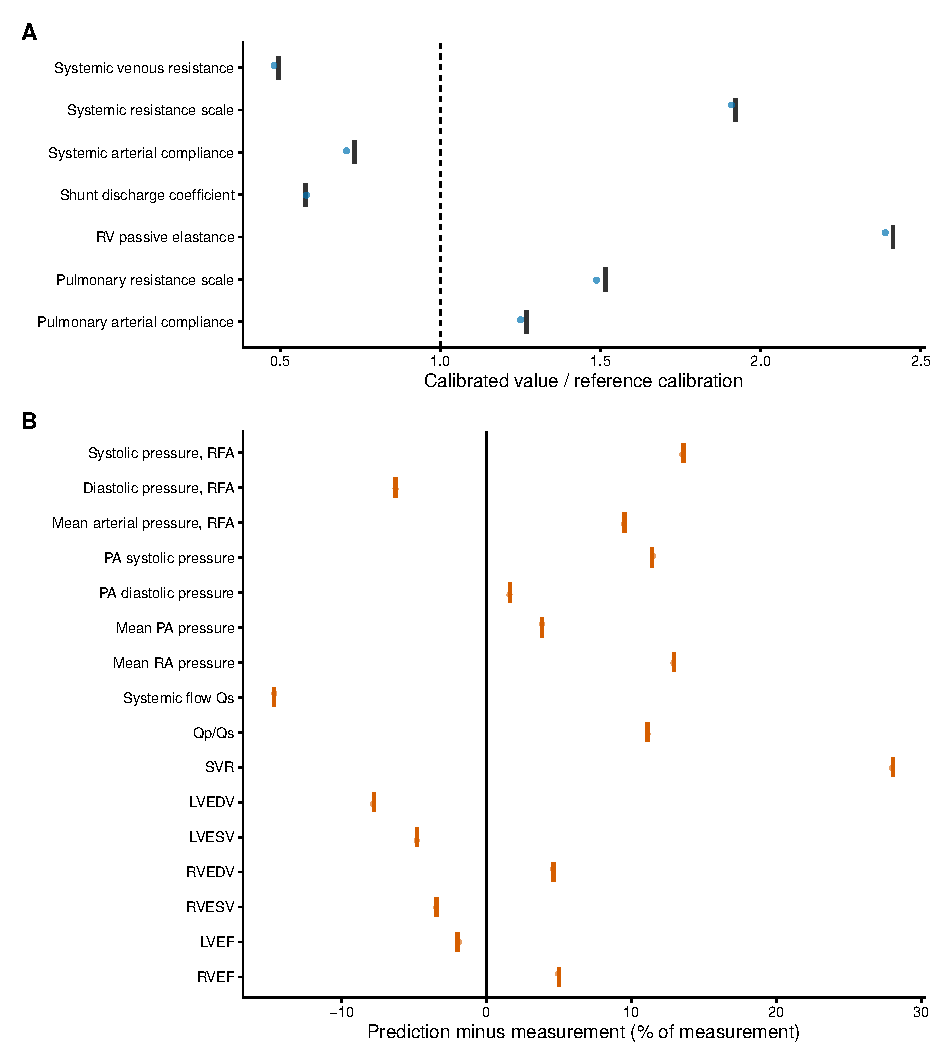
\includegraphics[width=\linewidth]{M6_noise.pdf}
\caption{Measurement-noise simulation ($n = 1$ recalibrated replicates). (A) Each calibrated parameter divided by its value in the reference calibration, one point per replicate; dashed line: reference. (B) Post-closure prediction minus measurement (\% of measurement), one point per replicate; the vertical line marks zero.}
\label{fig:noise}
\end{figure}
